\chapter{Experiments} \label{Experiments}

In this chapter, we define our experiment, the parameters involved in it for different agents and implementations and the final results of the simulation based on the implementation. The main focus of this chapter will be to characterize the complexity for different implementations mainly in terms of average time per move with different implementations and the result of tournament considered between the different agents. The main reason for the experiment is to validate our implementation and to compare the implemented agents including the random and semi-random agent baselines.

\section{Usage}

We use the console application to run all our experiments.

As an example, we provide the following arguments to the console application to simulate 100 games between Parallel-Minimax with a depth of 1 and Semi-Random agents on a game board of dimension 5x5:

\begin{lstlisting}[language=bash]
$dotnet run play -s1=parallelminimaxab -s2=semirandom -dimension=5 -depth=1 -sim -numsim=100
\end{lstlisting}

The aforementioned command produces the following output:

\begin{lstlisting}
===Results===
Player A : Parallel MinimaxAlgorithmABPruning won 99/100 games. Win rate : 99%. Average move time(ms) : 3.04
Player B : Semi-Random won 1/100 games. Win rate : 1%. Average move time(ms) : 1.05
Toal moves made across 100 games : 1781
Average total moves per game : 17
\end{lstlisting}

From the result above, we see that Parallel Minimax took \textbf{1781} moves across 100 games, with an average time of \textbf{3.04 ms} per move, and with an average win rate of \textbf{99\%}.

The link to the documentation for more sample commands for the console application can be found in Appendix \ref{app:consoleapp}.

In this thesis, the average time per move complexity can be defined as the average time taken by the agent to go through each move. The average is performed with respect to the total number of moves made by a particular agent in a game.

\section{Experiment 1 : Minimax depth tuning}

We first consider the implementation of the Minimax algorithm with the depth limited version, alpha-beta pruning version and the parallel version for different Quoridor board dimensions and demonstrate the time complexity of the implemented agents in terms of average time per move. 

For the following experiment, we run all of the 3 implemented variants of the Minimax algorithm including the alpha-beta and the parallel variant, we use the \textbf{Quoridor.ConsoleApp} console application, and simulate 100 games with different board and agent configurations against the semi-random strategy - a total of 36 times (3 variants of minimax x 3 depth x 4 dimensions).

\begin{figure}[!ht]
]
    \centering
    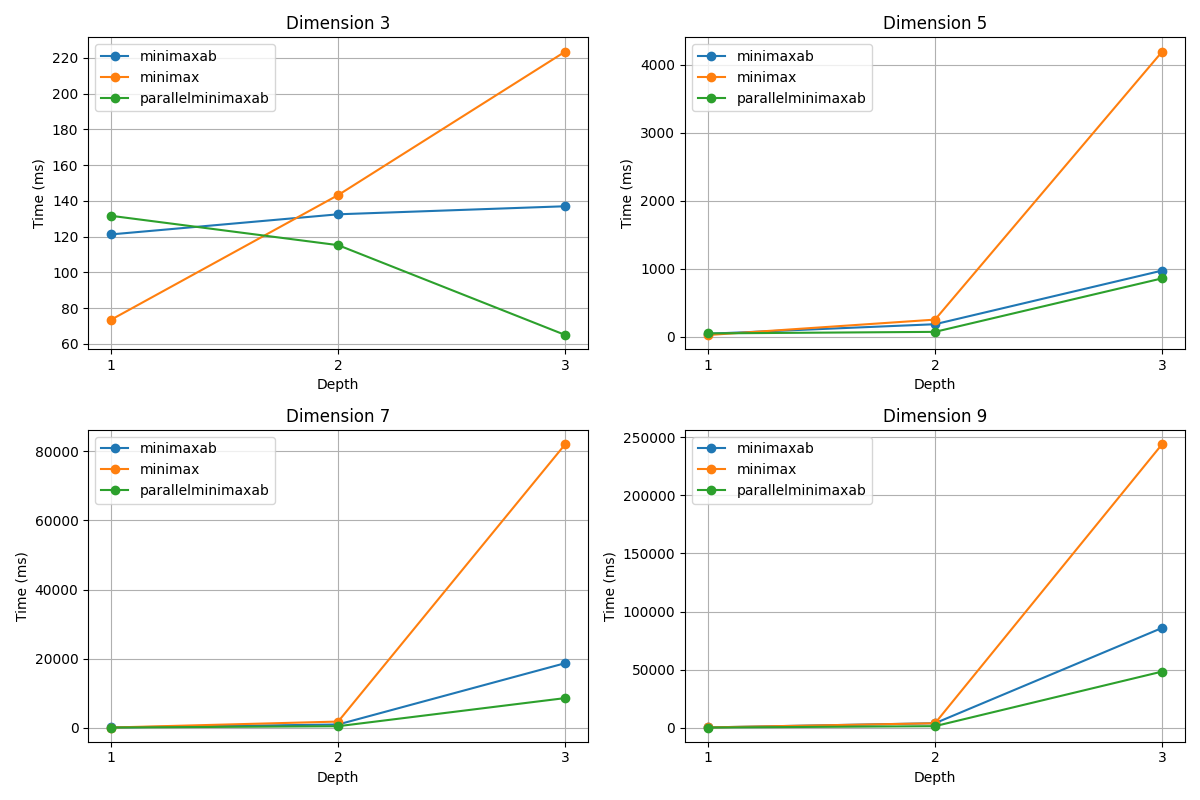
\includegraphics[width=\linewidth]{../img/performance.png}
    \caption{Average move time comparison between all 3 Minimax variants for different board sizes}
    \label{fig:minimax_performance_comp}
\end{figure}

In Figure \ref{fig:minimax_performance_comp}, we can see the average time per move of the Minimax algorithm along with its optimized variants on different board dimensions. In the figure, the dimension refers to the board dimension. For e.g., dimension 3 refers to a board size of 3x3 and so on. Considering the board of large dimension (e.g., 7 and 9), without further optimization, the complexity of implementing the Minimax algorithm for Quoridor is prohibitively high. For example, for depth 3, the move time complexity for the board with dimension 7 is 82 seconds and that for dimension 9 is 244 seconds.

From the figure, it can be inferred that for depth 1, the minimax algorithm without any further optimizations including alpha-beta or parallel implementation performs the fastest. The reason for this is straightforward, as for depth 1, the algorithm only evaluates one further move. In such case, there is not further improvement with alpha beta as we anyways need to evaluate all the nodes. The additional condition checking for the alpha beta implementation for this depth increases the average time per move without any gains. Similarly, the complexity of implementing the parallel algorithm outweighs the simple sequential evaluation hence increasing the time complexity per move without any impact on the performance.

However, for depths more than 1, it can be seen that the time complexity for each move considering alpha-beta pruning and further parallel implementation of the algorithm significantly improves as we increase the considered depth. Below, we have a table showing the improvement of the time complexity considering the minimax algorithm without any further optimization as the baseline.

\begin{table}[!ht]
    \centering
     \begin{tabular}{|c|c|c|c|}\hline
          & Depth 1 & Depth 2 & Depth 3\\ \hline 
          \textbf{Dimension: 3x3}  &    &    &     \\ \hline
          Minimax  &  1  &   1 &   1  \\ \hline
          Minimax alpha-beta &  1.8 &  0.92 &  0.61 \\ \hline
          Minimax alpha-beta parallel & 1.79 & 0.8& 0.29  \\ \hline
          \textbf{Dimension: 5x5}  &    &    &     \\ \hline
          Minimax  &  1  &   1 &   1  \\ \hline
          Minimax alpha-beta &  1.82 &  0.72 &  0.23 \\ \hline
          Minimax alpha-beta parallel & 2.06 & 0.27 & 0.20  \\ \hline
          \textbf{Dimension: 7x7}  &    &    &     \\ \hline
          Minimax  &  1  &   1 &   1  \\ \hline
          Minimax alpha-beta &  1.29 &  0.53 &  0.22 \\ \hline
          Minimax alpha-beta parallel & 1.05 & 0.25 & 0.10 \\ \hline
          \textbf{Dimension: 9x9} &    &    &     \\ \hline
          Minimax  &  1  &   1 &   1  \\ \hline
          Minimax alpha-beta &  1.06 &  1 &  0.35 \\ \hline
          Minimax alpha-beta parallel & 0.43 & 0.33 & 0.19  \\ \hline
     \end{tabular}
     \caption{Relative move-time complexity compared to the baseline minimax algorithm}
     \label{tab:complexity}
 \end{table}

In Table \ref{tab:complexity}, we present the relative move time complexity of the different algorithms with reference to the minimax algorithm for the same depth. Here, we can see that, especially for depth 2 and depth 3, the minimax algorithm, when using the alpha beta pruning and further parallel implementation takes significantly less time. This is especially relevant when considering the large dimension of the Quoridor board as the move time complexity is significantly high. Here, optimization is required for running the algorithm in relatively manageable time.

So, in the experiments that follow, we will use the Parallel Minimax algorithm.

\section{Experiment 2 : 3x3 board}

In this section, we perform various simulations to find out the best parameters for the \gls{MCTS} algorithm, and use those to run head-to-head simulations between all agents to find out the best performing one for the 3x3 game board.

\subsection{MCTS parameter tuning}

The main aim of this experiment is to tune the parameters in the MCTS algorithm, namely the number of iterations and the exploration parameter. Given a relatively small size of the board, each move has a significant impact on the result, where a single miscalculation can lead to an immediate loss. For example, Figure \ref{fig:3x3InitialGameState} depicts the initial game state for the 3x3 configuration. Player A makes a move \texttt{b2} resulting in the game state depicted by Figure \ref{fig:3x3b2movebyA}. Player B now can immediately win with the move \texttt{a2} (it jumps over player A). Considering this, we choose a large number of game iterations, \textbf{500} for MCTS. Higher iteration count allows for a comprehensive evaluation of the game states, accounting for the strategic depth required in the tight confines of a 3x3 board where tactical blunders are less forgivable and can lead to a loss, allowing the algorithm to recognize and avoid simplistic heuristics that may overlook such critical missteps as depicted in figure \ref{fig:3x3BadMove}

\begin{figure}[!ht]
    \begin{subfigure}{0.3\textwidth}
      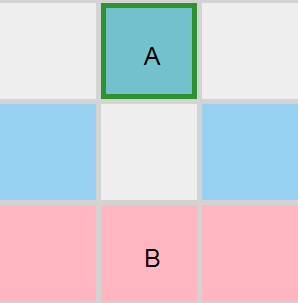
\includegraphics[width=\textwidth]{../img/GameBoard/3_3_board_start.png}
      \caption{Initial game state}
      \label{fig:3x3InitialGameState}
    \end{subfigure}
    \hfill
    \begin{subfigure}{0.3\textwidth}
      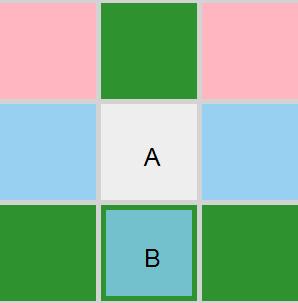
\includegraphics[width=\textwidth]{../img/GameBoard/3_3_mcts_move.png}
      \caption{b2 move by player A}
        \label{fig:3x3b2movebyA}
    \end{subfigure}
    \caption{First bad move by player A leading to a (possible) loss}
\label{fig:3x3BadMove}
\end{figure}

Using \textbf{500} iterations, we conduct an experiment by playing the MCTS agents against two different opponents, A* and Minimax with varying exploration parameters. In this experiment, we consider the minimax algorithm with depth of 2 and simulate 50 games for each exploration parameter. We vary the exploration parameter from 0.6 to 1.4 with a interval of 0.1. As we see on Figure \ref{fig:3x3MCTSTuningAStar}, MCTS algorithm with an exploration parameter of \textbf{0.6} won \textbf{100\%} of the games against the \textbf{A*} algorithm and an average of \textbf{74\%} against the \textbf{Minimax} algorithm (with a depth of 2).

\begin{figure}[!ht]
    \begin{subfigure}{0.5\textwidth}
      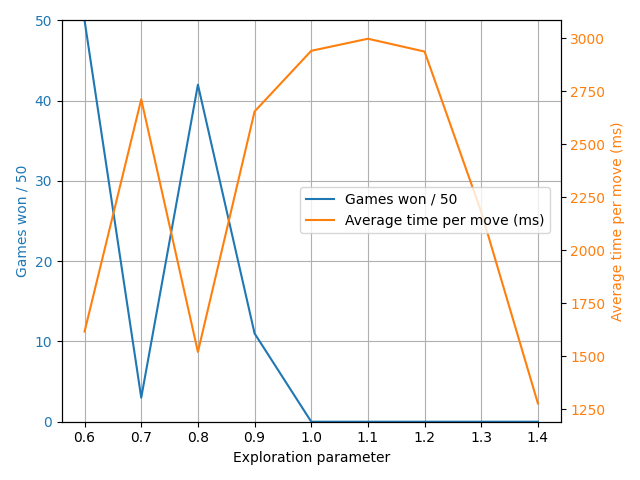
\includegraphics[width=\textwidth]{../img/mcts_exploration_param_grid_search_3_astar.png}
      \caption{MCTS vs A*}
      \label{fig:3x3MCTSTuningAStar}
    \end{subfigure}
    \hfill
    \begin{subfigure}{0.5\textwidth}
      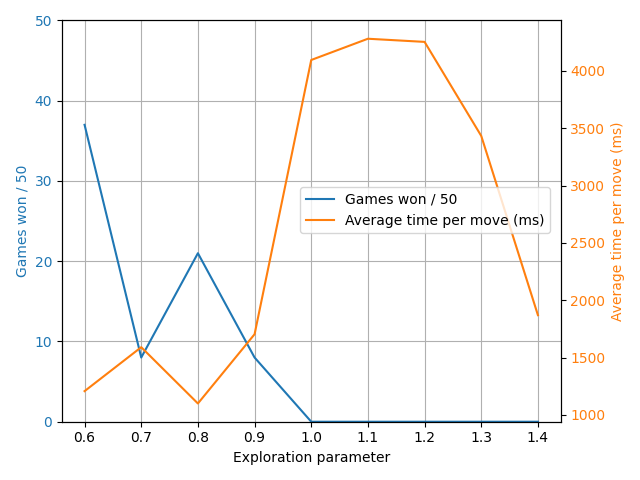
\includegraphics[width=\textwidth]{../img/mcts_exploration_param_grid_search_3_minimax.png}
      \caption{MCTS vs Minimax}
        \label{fig:3x3MCTSTuningMinimax}
    \end{subfigure}
    \caption{Average time per move and win rates of MCTS agent running 500 iterations with varying exploration parameter for board size 3x3}
\label{fig:3x3MCTSTuning}
\end{figure}

Furthermore, as depicted by the graphs in Figure \ref{fig:3x3MCTSTuning}, MCTS algorithm loses all games against the two opponents when the exploration parameter is greater than 1. A parameter greater than 1 excessively prioritizes \textbf{exploration} of states with very few simulations, leading to a neglect on promising strategies already discovered by the MCTS algorithm. This can cause the algorithm to overlook immediate threats or miss direct paths to victory, as evidenced by the total losses incurred at higher parameter values on Figure \ref{fig:3x3MCTSTuning}. In contrast, an exploration parameter less than 1 indicates a balanced approach that weighs the value of \textbf{exploiting} well-performing moves against the potential benefit of exploring new moves. This balance is particularly critical on the small 3x3 board, where each decision carries significant weight. Therefore, an exploration parameter value below 1 is preferred for a 3x3 Quoridor board, as it ensures that the algorithm maintains a focus on exploiting successful strategies while still considering any potential novel moves, leading to more consistent and strategic game play.

\subsection{Results}
In Table \ref{tab:agent_eval_3x3}, we present the tournament result for the agents for the board dimension 3x3 and present the results. For the simulation, we ran the experiment 1000 times between different agents. For the minimax agent, we considered the depth of 2. For \gls{MCTS} agent, we considered the determined optimal exploration parameter of 0.6 and 500 \gls{MCTS} simulations per move.

A value $V_{i,j}$ for agents $i$ and $j$ refers to the average win rate out of 1000 simulations with agent $i$ as player A and agent $j$ as player B.

With these parameters, we can now compare various agents on a board of dimension 3x3.

\begin{table}[!ht]
    \centering
     \begin{tabular}{|c|c|c|c|c|c|}\hline
    \backslashbox{p1}{p2}            & Random & Semi-Random & A*  & Minimax & MCTS \\ \hline 
    Random      &        &    31.3     & 6.6 &   5.3   &  0   \\ \hline
    Semi-Random &   73.5 &             & 11.5&   10.2  &  0  \\ \hline
    A*          &   92.2 &    90.2     &     &   0     &  0   \\ \hline
    Minimax     &   92.4 &    88.9     & 8.2 &         &  0   \\ \hline
    MCTS        &   90   &    74.3     &  100 &   74    &      \\ \hline
     \end{tabular}
     \caption{Agent comparison for dimension 3x3. The values in the
table represent the total win percentage of the agent in the row of the table when competing against the agent in the column of the table.}
     \label{tab:agent_eval_3x3}
 \end{table}

\section{Experiment 3 : 5x5 board}

Following the results of the 3x3 board experiment as presented in Table \ref{tab:agent_eval_3x3}, we would also like to find out the ideal \gls{MCTS} parameters for the 5x5 variant and run a head-to-head tournament betweeen all our implemented agents.

\subsection{MCTS parameter tuning}

For this experiment, we consider a Quoridor board of size 5x5 and play against a Minimax agent with a depth 2 and like the previous scenario, perform 50 experiments per parameter we are interested in.

First, we perform a grid search to find the ideal number iterations for the 5x5 board, using average win-rate as our deciding factor. We iterate over a range of 30 to 240 with an interval of 30 and run 50 simulations, all while using a theoretical optimal exploration parameter of $\sqrt{2}$ \citep{kocsis2006bandit}.

\begin{figure}[!ht]
    \centering
    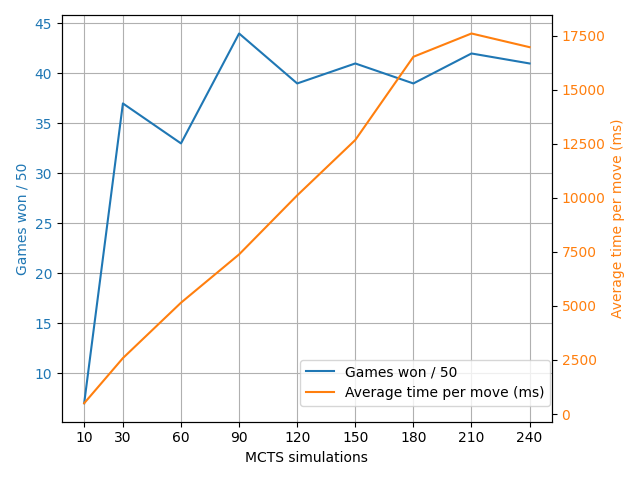
\includegraphics[width=0.7\linewidth]{../img/mcts_simulation_grid_search.png}
    \caption{Average time per move and win rates of MCTS agent with varying simulations for board size 5x5}
    \label{fig:mcts_simulations}
\end{figure}

In Figure \ref{fig:mcts_simulations}, we see that after 90 simulations, the additional marginal number of game won does not increase, although the time per move increases. Hence, optimizing the number of simulations can be important to limiting the complexity of the \gls{MCTS} agent.

\begin{figure}[!ht]
    \centering
    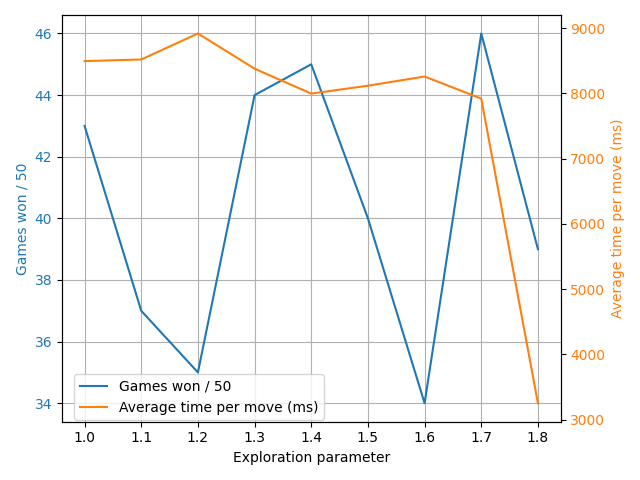
\includegraphics[width=0.7\linewidth]{../img/mcts_exploration_param_grid_search.png}
    \caption{Average time per move and win rates of MCTS agent with varying exploration parameter for board size 5x5}
    \label{fig:mcts_exp_simulations}
\end{figure}

Likewise, in Figure \ref{fig:mcts_exp_simulations}, we use 90 iterations we deduced from Figure \ref{fig:mcts_simulations} to find the optimal exploration parameter based on the number of games won varied with different exploration parameters. From Figure \ref{fig:mcts_exp_simulations}, we see that with an optimal exploration parameter of \textbf{1.7}, the win rate for the agent is high i.e 46 wins out of 50 games.

\subsection{Results}
 
 Firstly, we can observe that the Random agent, as expected, does poorly against all other agents. However, in the 3x3 board, the Random agent still wins a third of the time again Semi-Random agent and a few times against the even the A-star and the Minimax agents. From the table, it can also be observed that the \gls{MCTS} agent performs the best in the 3x3 board as it almost does not lose any games against the any other agents.

\begin{table}[!ht]
    \centering
     \begin{tabular}{|c|c|c|c|c|c|}\hline
     \backslashbox{p1}{p2} & Random & Semi-Random & A*  & Minimax & MCTS \\ \hline 
    Random      &        &    5.8      &  0  &   0     &   0  \\ \hline
    Semi-Random &   93.6 &             & 0.3 &   1.9   &  3.3 \\ \hline
    A*          &   100  &    99.7     &     &   22.7     & 73.3 \\ \hline
    Minimax     &   99.9 &    99.4     & 87.3 &         & 33.3 \\ \hline
    MCTS        &   100  &    100      & 56.7&   92    &      \\ \hline
     \end{tabular}
     \caption{Agent comparison for dimension 5x5. The values in the
table represent the total win percentage of the agent in the row of the table when competing against the agent in the column of the table.}
     \label{tab:agent_eval_5x5}
 \end{table}

 In Table \ref{tab:agent_eval_5x5}, we present the result of the tournament when considering a Quoridor board of dimension 5. For this board dimension, we again consider the total number of simulation runs as 1000. For the minimax agent, we considered the depth as 2. For the \gls{MCTS} simulation, we considered the determined optimal exploration parameter of 1.7 and ran 90 simulations per move.
 
 From the table, we can observe that considering a board of a larger dimension, both the Random and the Semi-Random agents perform poorly since they require a large number of good moves in a sequence to win, which is less-likely to happen. From the table, we can also see that the \gls{MCTS} algorithm performs best against all the algorithms, winning more than 90\% of its games except for the A-star agent where it wins more than half of its games. Another surprising factor is that the A-star algorithm which only considers the distance from the start position and end position as the main cost functions performs much better than the minimax algorithm.  

\section{Experiment 4: 7x7 board}

For the \gls{MCTS} agent, since the average move time was 34.4 seconds with the available simulation hardware, we could only perform 100 simulations. Additionally, the simulation run time also prevented us from using an optimized parameter. Hence, we used the theoretical optimal parameter of $\sqrt{2}$ \citep{kocsis2006bandit} for this dimension. For the minimax agent, we considered the implementation with depth 2. 

\begin{table}[!ht]
    \centering
     \begin{tabular}{|c|c|c|c|c|c|}\hline
\backslashbox{p1}{p2}& Random & Semi-Random & A*  & Minimax & MCTS \\ \hline 
    Random      &        &    0.2        &  0  &   0     &  0    \\ \hline
    Semi-Random &   99.6 &             & 0.2 &  0.7    &  0.2 \\ \hline
    A*          &   100  &    99.7     &     &   18.2     &  2    \\ \hline
    Minimax     &   100  &    99.3     & 79.8 &         & 58 \\ \hline
    MCTS        &    100    & 100  &  3   &        44 &      \\ \hline
     \end{tabular}
     \caption{Agent comparison for dimension 7x7. The values in the
table represent the total win percentage of the agent in the row of the table when competing against the agent in the column of the table.}
     \label{tab:agent_eval_7x7}
 \end{table}
 
In Table \ref{tab:agent_eval_7x7}, we illustrate the result of the tournament when considering a board of dimension 7x7. For this dimension we also ran 1000 simulations for all the agents except for the \gls{MCTS} agent. 

Here, the performance of the random agent is significantly worse compared to the previous boards as it fails to win any games against A-star, minimax and MCTS agents. Unlike the previous smaller boards, in this instance, the minimax algorithm performs much better against A-star algorithm as it wins almost all of its games. From this, we can conclude that the strategical play with the minimax algorithm for larger board is much more significant than the simple cost function oriented traversal strategy of the A-star algorithm.
 
From the above tournament simulation presented in Table \ref{tab:agent_eval_7x7}, we can conclude that the board dimension does have an effect on the strategy that might be used. For board of smaller dimensions such as 3 and 5, simpler strategies such as  random and semi-random in some cases can be enough to get some wins against more strategical agents such as the minimax agent. However, as the board dimension gets higher, the required strategy is very prominently visible as semi-random and random agents win almost no games against the other agents.